\section{Koordinationsverbindungen I -- Kristallfeldtheorie}
\authors{Isabelle Schulte-Herbrüggen, Jonas R. Stöckmann}
\subsection{Allgemeines}

Die Koordinationsverbindungen wurden 1893 von Alfred Werner erstmals konsistent beschrieben. 
\cite{Werner1893}
Sie bestehen aus einem Zentralatom, welches sich in der Mitte des Komplexes befindet und von Liganden umgeben ist.
 Bei Liganden handelt es sich um Moleküle oder Anionen mit mindestens einem freien Elektronenpaar. Die Koordinationszahl des Komplexes gibt die Anzahl der Liganden beziehungsweise die Anzahl der an das Zentralatom koordinativ bindenden 
Haftatome der Liganden an. 
Diese Aussage konnte mithilfe experimentell ermittelter Werte der molaren Leitfähigkeit unterschiedlicher Komplexe getroffen werden.
So hat NaCl eine molare Leitfähigkeit von 123 $\frac{cm^3}{\Omega*mol}$, bei einem freien Chloridion. $CoCl_3\cdot5NH_3$ hat eine molare Leitfähigkeit von 261$\frac{cm^3}{\Omega*mol}$, was auf zwei freie Chloridionen schließen lässt. Daraus kann man folgern, dass anstatt des anfänglichen $CoCl_3\cdot5NH_3$ nur noch ein $ [Co(NH_{3})Cl]^{2+} $-Ion vorliegt, was zeigt, dass ein Chloratom gebunden sein muss.
\subsection{Kristallfeldtheorie}
In der Kristallfeldtheorie wird das Zentralatom quantenmechanisch betrachtet,
während das Radialfeld von Ladungsträgern, welches das Zentralatom umgibt, klassisch betrachtet wird. Auch die Wechselwirkungen werden klassisch elektrostatisch betrachtet.
Dabei ist das Zentralatom in einem kugelsymmetrischen Feld gleichmäßig verteilter Ladungen lokalisiert.
Die Liganden werden später als Punktladungen betrachtet.
Bei dem Zentralatom handelt es sich meist um ein Metallatom beziehungsweise -ion mit Valenz-$d$-Orbitalen.
Wenn sich ein Zentralteilchen mit 3$d$-Konfiguration in dieser geladenen, kugelsymmetrischen Umgebung  befindet, führt dies dazu, dass die Energien aller 3$d$-Orbitale auf gleiche Weise angehoben werden. Daraufhin erfolgt eine Aufspaltung der Energieniveaus, abhängig von der räumlichen Anordnung der Liganden.
\subsection{Oktaeder}
Bei der räumlichen Anordnung der Liganden in der Oktaeder-Symmetrie werden das $d_{z^2}$($e_g$-Orbital) und das $d_{x^2-y^2}$ ($t_{2g}$-Orbital) um $\frac{3}{5}\Delta_{O}$  angehoben, während das $d_{xy}$, $d_{yz}$ und das $d_{xz}$ ($t_{2g}$-Orbitale) um $\frac{2}{5}\Delta_{O}$ auf ein energetisch günstigeres Niveau gebracht werden. 
Dies kann durch die Abstoßung der $d$-Orbitale und Punktladungen begründet werden.
Dabei ist $\Delta_{O}$ von verschiedenen Faktoren abhängig. Dazu gehören die jeweiligen Liganden, das Zentralatom, die Koordinationszahl, die Koordinationsgeometrie und der Abstand von Zentralatom und Ligand zueinander.

Im Spezialfall der $ d^{8} $- und $ d^{9} $-Systeme sind die beiden HOMOs, wie in Abbildung 1.1 dargestellt, jeweils  einfach besetzt.
Der Zustand ist somit entartet und instabil. Diese Entartung wird aufgehoben, indem die Bindungslängen entlang der $z$-Achse deutlich verlängert und die ursprüngliche Symmetrie des Komplexes aufgehoben wird.
Entfernt man die Liganden, welche auf der $z$-Achse liegen, unendlich weit voneinander, entsteht im Grenzfall eine quadratisch planare Struktur.

Durch diesen Vorgang werden die HOMOs in zwei verschiedene Energieniveaus aufgespalten. Das $d_{z^2}$-Orbital ist nun ein voll besetztes und energetisch günstigeres HOMO, während das $d_{x^2-y^2}$ nun unbesetzt ist (siehe Abbildung 1.1). Durch die Veränderungen dieser energetisch ungünstigeren Energieniveaus ändern sich auch die Energieniveaus des $d_{xy}$, welches angehoben wird. $d_{xz}$ und $d_{yz}$ werden hingegen stabilisiert.
Dies bezeichnet man als Jahn-Teller-Effekt.

\begin{dsafigure}
\centering
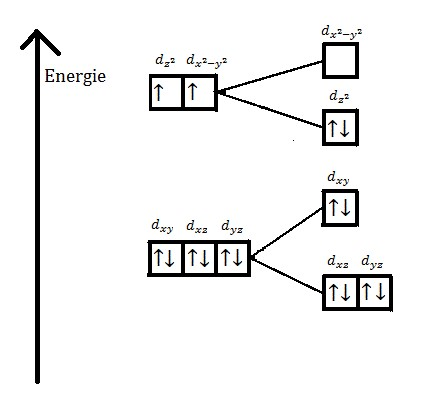
\includegraphics[scale=0.567]{Energieniveauskristallfeldtheorie.jpg}
\caption{Links ist die Aufspaltung der Orbitale im Oktaederfeld dargestellt, rechts die Aufspaltung durch Elongation der Bindungen in z-Richtung.}
\label{dsafigure:beispiel}
\end{dsafigure}

\subsection{Tetraeder}
Die Tetraeder Symmetrie ist äquivalent zur Würfelsymmetrie, da gilt: $\Delta_{t}=\frac{1}{2}\Delta_{w}$.
\cite{Koordinationsverbindung}
Bei einem Tetraeder geht die $z$-Achse durch zwei gegenüberliegende Kanten. Die größte Abstoßung findet auf Grund von elektrostatischer Wechselwirkung zwischen zwei Achsen statt. Aus diesem Grund werden in diesem Fall das $d_{xy}$, $d_{xz}$ und das $d_{yz}$-Orbital um $\frac{2}{5}\Delta$t angehoben, während das $d_{z^2}$ und das $d_{x^2 - y^2}$ Orbital um $\frac{3}{5} \Delta_t$ stabilisiert werden. In diesem Fall ist $\Delta _{t}$ allerdings größer als bei einem Oktaeder.
